
\documentclass[en]{ujdpl}

\usepackage[polish]{babel}
\usepackage[utf8]{inputenc}
\usepackage{ae}

\usepackage[T1]{fontenc}

\usepackage[justification=centering]{caption}

\usepackage{url}
\usepackage{latexsym}
\usepackage{textcomp}

\usepackage{titlesec}
\usepackage{graphics} % wlaczanie grafik
\usepackage{wrapfig}

\usepackage{color} % kolory
\usepackage{floatflt}
\usepackage{bookmark}
\frenchspacing
\usepackage{indentfirst}

% dodatkowe pakiety
\usepackage{amsmath}
\usepackage{multirow}
\usepackage{enumerate}
\usepackage{listings}
\usepackage[usenames,dvipsnames]{xcolor}
\lstloadlanguages{xml}

\hyphenpenalty=100000

\definecolor{listinggray}{gray}{0.9}
\definecolor{lbcolor}{rgb}{0.9,0.9,0.9}
\lstset{
	backgroundcolor=\color{lbcolor},
	tabsize=4,
	rulecolor=,
	language=xml,
        basicstyle=\scriptsize,
        upquote=true,
        aboveskip={1.5\baselineskip},
        columns=fixed,
        showstringspaces=false,
        extendedchars=true,
        breaklines=true,
        prebreak = \raisebox{0ex}[0ex][0ex]{\ensuremath{\hookleftarrow}},
        frame=single,
        showtabs=false,
        showspaces=false,
        showstringspaces=false,
        identifierstyle=\ttfamily,
        keywordstyle=\color[rgb]{0,0,1},
        commentstyle=\color[rgb]{0.133,0.545,0.133},
        stringstyle=\color[rgb]{0.627,0.126,0.941},
}


\lstdefinelanguage{JavaScript}{
  keywords={typeof, new, true, false, catch, function, return, null, catch, switch, var, if, in, while, do, else, case, break, this},
  keywordstyle=\color{blue}\bfseries,
  ndkeywords={class, export, boolean, throw, implements, import},
  ndkeywordstyle=\color{}\bfseries,
  identifierstyle=\color{black},
  sensitive=false,
  comment=[l]{//},
  morecomment=[s]{/*}{*/},
  commentstyle=\color{purple}\ttfamily,
  stringstyle=\color{red}\ttfamily,
  morestring=[b]',
  morestring=[b]"
}

\lstset{
   language=JavaScript,
   backgroundcolor=\color{listinggray},
   extendedchars=true,
   basicstyle=\footnotesize\ttfamily,
   showstringspaces=false,
   showspaces=false,
   numbers=left,
   numberstyle=\footnotesize,
   numbersep=9pt,
   tabsize=2,
   breaklines=true,
   showtabs=false,
   captionpos=b
}


% paragraph gap:
\setlength{\parskip}{0.5\baselineskip plus 0.5ex minus 0.2ex}

%---------------------------------------------------------------------------

\author{Sebastian Poręba}
\shortauthor{Sebastian Poręba}

\title{Comparison of 3D physics engines}

\shorttitle{Comparison of 3D physics engines}

\thesistype{Praca magisterska}

\supervisor{dr hab. Paweł Węgrzyn}
\consultant{mgr Bartosz Porębski}

\date{2013}

\faculty{Wydział Fizyki, Astronomii i Informatyki Stosowanej}

\acknowledgements{I would like to thank my advisors Paweł Węgrzyn and Bartek Porębski. Also I need to thank Collin Hover and Ibon Tolosana for their valuable insights and help with tests.}

%---------------------------------------------------------------------------

\begin{document}

\titlepages

\setcounter{tocdepth}{1}
\tableofcontents

\clearpage

\newcommand{\sectionbreak}{\clearpage}

\chapter{Introduction}
\label{cha:introduction}

The main objective of presented project is the implementation of parts of 3D engine in a browser environment. Parts of engine are analysed side-by-side with parallel engine compiled from C++. The objective of analysis is comparison of performance and description of possible issues related to the limited browser resources and dynamic features of JavaScript.

At the moment of writing majority of games are developed with C++ and usually DirectX. These technologies are mature and have excellent performance. Features of the language give flexibility and high-level solutions to effectively manage application (e.g. operator overloading, multiple inheritance) and allow to fine-tune internals of application to achieve best execution times. For games with high budget\footnote{Grand Theft Auto V, released in 2013 had a budget of \$137 millions - http://www.gamesindustry.biz/articles/2013-02-01-gta-v-dev-costs-over-USD137-million-says-analyst} C++ is an obvious choice for having the best possible result.

However, in parallel to AAA game industry casual and independent games sector is growing. In 2013 market is expected to be worth \$8.64 billions in total. Total of 2.4 billion tablets and smartphones with casual games capabilities will be reached before the end of 2013. These games are less focused on creating cutting edge graphics and physics simulations and more on overall experience and social interactions.

JavaScript is a scripting language not designed to perform high-load computations. However, at present it is the only language widely supported by all browsers. With all it's advantages and quirks is the only choice available for programmers.\footnote{Currently two new languages are worked on - Dart by Google and TypeScript by MicroSoft. However, to enable cross-compilation to JavaScript, paradigm of these languages is similar and work is focused mainly on better IDE support.}

While suffering from design issues, JavaScript provides a complete environment that makes development very easy for both beginner and advanced programmer. Two very important components of every application are provided out of the box - rendering system and networking in browser, designed for HTML pages to carry mainly text information are still suitable for gaming. Creation of simple 2D game is often a matter of few hundred lines of code responsible for transferring user input to positions of sprites defined in CSS. This is clearly visible during competitions like JS13kGames\footnote{http://js13kgames.com/} where all game assets and code have to be fitted into 13kB package. 

Many projects varying from server side solutions\footnote{http://nodejs.org/}\footnote{http://googlecreativelab.github.io/coder/} to hardware developer boards\footnote{http://www.espruino.com/} are taking advantage of this simplicity. From the perspective of game development, it is unlikely at the time of writing that AAA game may be created to run in browser. However, growing segments of casual, independent and social games are already targeting web as a platform.

\section{Influence on distribution process}

Traditionally, games are often still sold in physical boxes and some update system is always incorporated to patch any bugs appearing after initial release. Systems like Steam\footnote{http://store.steampowered.com/} are making this process easier but still suffer from necessity to install a game on hard drive.

Creating application that works in browser simplifies distribution significantly. All assets and code are downloaded each time user enters a website, so no update system is necessary - all users always play the newest version. Usually browser games are monetised differently than traditional titles. Playing basic version is usually free and earnings come from either ads or premium content. This is completely new approach, present also in MMO\footnote{Massive Multiplayer Online} games. It resulted in psychological research on leveraging compulsive behaviours to maximise profits\footnote{http://www.emcneill.com/exploitative-game-design-beyond-the-f2p-debate/}.

Working in browser gives access to all social network of user, so incorporation of Twitter or Facebook based features is very simple - which boosts promotion of game. It also enables, morally questionable, target of people not able to install games on company issued computer. Disallowing games in browsers is far more complicated task for administrator, similar to blocking ads or mature content.

Lastly, web is better suited to run easily on all platforms. Browser is a layer of abstraction that makes transparent for application, whether it runs on any traditional operating system, gaming console or mobile device. Of course  performance and screen size should be taken under consideration, but ability to write one codebase that runs on multiple devices led already to projects that package JavaScript applications as native ones\footnote{http://phonegap.com/}, greatly reducing development costs for growing variety of phones and tablets.

\begin{figure}[h!]
  \caption{Game created with ImpactJS}
  \label{img:impactjs}
  \centering
	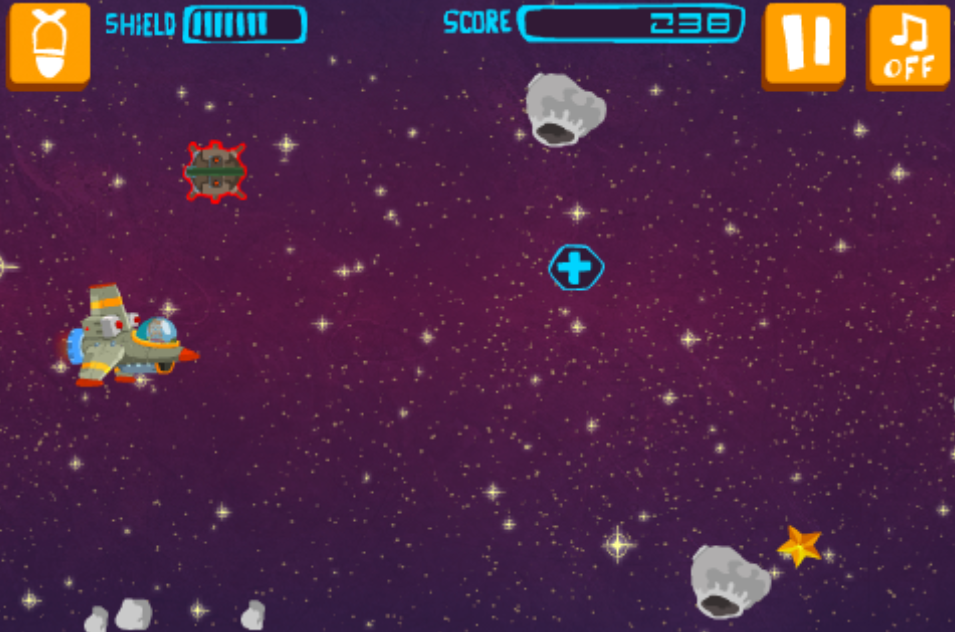
\includegraphics[width=12cm]{summary/impactjs.png}
\end{figure}

Multiple open-source and commercial game engines are created lately. Examples worth mentioning are ImpactJS\footnote{http://impactjs.com/}, Turbulenz\footnote{http://biz.turbulenz.com/turbulenz} and Isogenic Engine\footnote{http://www.isogenicengine.com/}.


\begin{figure}[h!]
  \caption{Game created with Isogenic Engine}
  \label{img:isogenic}
  \centering
	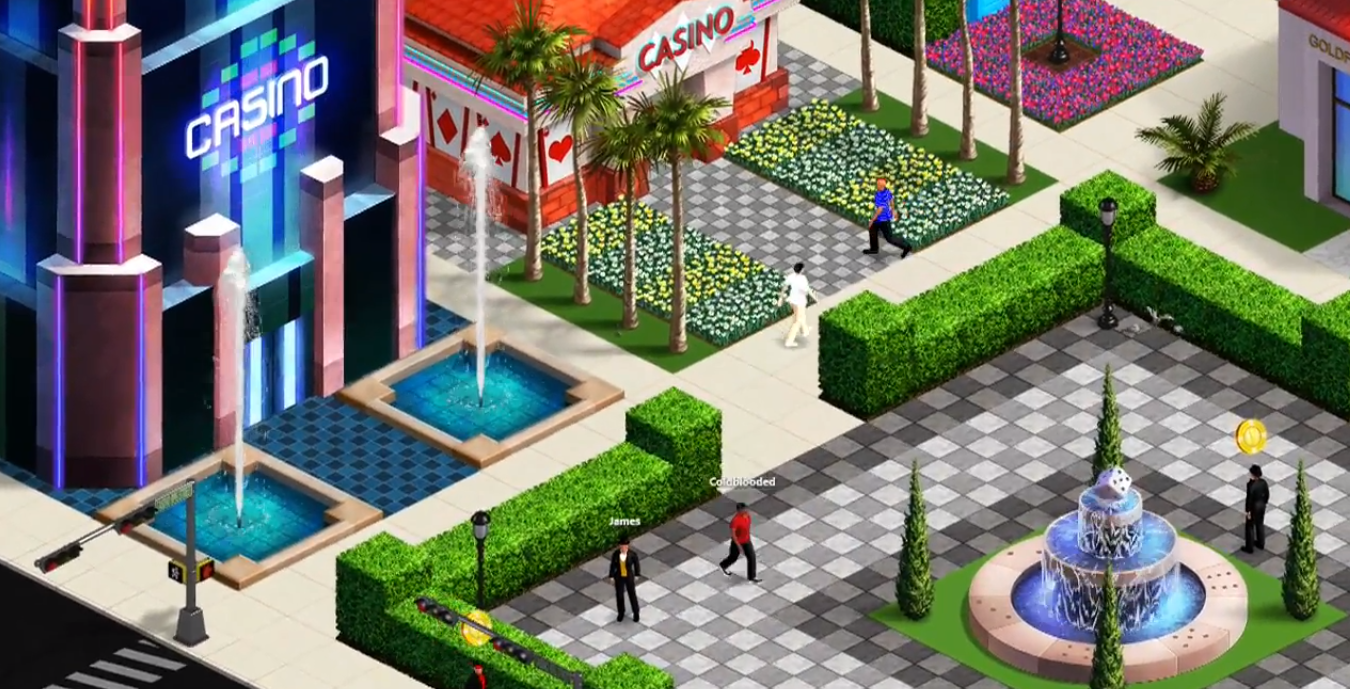
\includegraphics[width=12cm]{summary/isogenic.png}
\end{figure}

Very important and growing sector are interactive 3D arts with two major targets - music videos and commercials. They are uniquely available only in browsers as a very viral extensions of normal marketing. One of the first occurrences of this technology was video for Rome music group: "3 dreams of black"\footnote{http://www.ro.me/}. Project allows to move the camera while animated 3D story is rendered alongside music. After movie is over user is allowed to create 3D models that are later incorporated into experiences of other people watching. This way interactions and social element are enabled in what used to be one-way transmission of art form. 

\begin{figure}[h!]
  \caption{Screenshot from "3 dreams of black"}
  \label{img:rome}
  \centering
	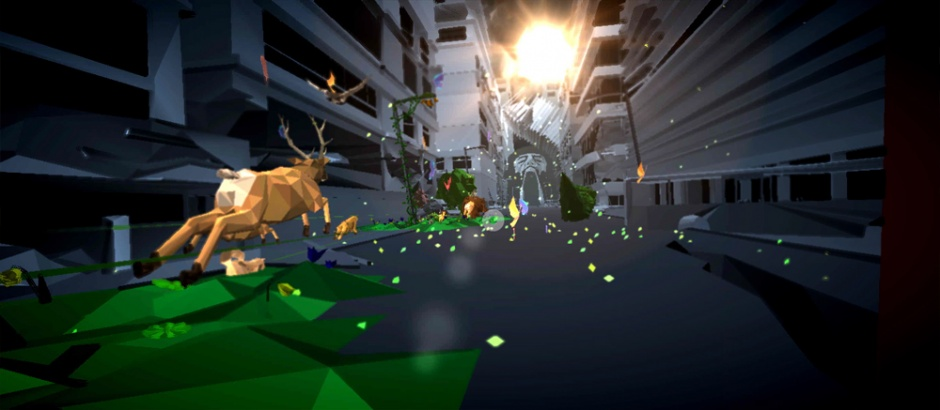
\includegraphics[width=12cm]{summary/rome.jpg}
\end{figure}

\section{Technology}

Browser-based engine is implemented in JavaScript and analyzed in V8 engine. V8 is maintained by Google and is used in Google Chrome browser. Executable examples are compiled using gcc compiler and are runned on the same platform. For additional comparison Emscripten project is used to automatically generate JavaScript and measure if automated conversion may be as effective as writing code by hand.

Project is based on conference sessions and announcements authored by V8 programmers regarding performance of JavaScript applications. Analysis of available materials is a topic of Chapter 2, where internals of modern engines for dynamic languages are briefly explained.

Chapter 3 covers particles often used to simulate loosely connected systems like smoke, fire, fog, etc. It shows techniques of memory allocation and garbage collection that help improve performance. Two particle systems are presented - one with high memory allocation that is expected to cause performance issues and second one, improved by usage of object pools.

Chapter 4 is focused on sphere collision detection and reaction, with both naive solution and space partitioning using Octree. This benchmark shows application with high CPU usage and relatively simple math computations. Because of this simplicity, collision detection with spheres is almost always used as a preliminary method of eliminating collision between objects. Only if bounding spheres are colliding more complex and expensive algorithms are used to determine real state of such pair.

Systems presented in chapters 3 and 4 are not targeted to be full physics engines. They are however representative to general concepts encountered in every game.

Chapter 5 describes Emscripten, project aimed to convert complete C++ projects to JavaScript. Related library, asm.js, is presented with overview of architectural choices that lead to better performance. Generated code is compared to the one created in previous chapters and execution times of all benchmarks is compared and briefly explained.

Last chapter is summary of all achieved results. Limitations of JavaScript engines are presented alongside future possibilities for gaming industry. 

Benchmarks are by no means a complete physics system and are not representing current state of the art of physics algorithms. They are aimed to resemble optimal algorithms in used methods and complexity, so that benchmarks reflect how actual engine is using memory and computing power.


\chapter{Overview of JavaScript and V8 engine architecture}
\label{cha:overview}

Historically, JavaScript was considered an untyped language, meaning that values had no types attached to variables, either by the programmer or the compiler. All variables were of a single, unified type, and procedures called unboxing and boxing, performed before and after each operation on a variable, ensured that it was properly used on the machine code level. The complete code source was sent from the server to the browser and was parsed and executed on the fly. Without types attached to variables, all functions were polymorphic and unstable, since parameters may have carried any type of variable. To solve this problem, the source code of the function was parsed every time it was called, each time generating a machine code based on current parameters and variables in scope. This approach, called interpretation, is still present in JavaScript engines, and used whenever variables do not match set criteria of stability described later in this chapter.

This paper uses as an engine of choice V8 Crankshaft. This choice was made, because it is the only engine available at the moment which provides direct command line access, enabling the precise performance measurements of code parsing and execution, without browser context and overhead. The executable file of V8 (named d8) is compiled with consideration to the target platform.

\section{JIT compilation -- tracking variable types}
\label{sec:JIT}

As it was mentioned before, initially JavaScript was treated as an untyped language. With the release of SpiderMonkey in Firefox 3.5 in 2009, the situation changed. The first Just-In-Time compiler for JavaScript, TraceMonkey, was created. Based on the works of Prof. Dr. Michael Franz on TraceTrees \footnote{http://www.michaelfranz.com/} JIT compiler collected all paths that the interpreter took with specific types of variables. A path could split into different methods or if statements. Whenever part of the code was executed often enough, the path was marked as hot, and the compiler optimised it for given types. If a single path was traversed with a different set of types, the compiler could generate another version of the optimised code. When the path turned out to be highly polymorphic, optimised versions were removed and the interpreter was used as a fallback.
Initial reports show speedups between 20x to 40x \footnote{http://arstechnica.com/information-technology/2008/08/firefox-to-get-massive-javascript-performance-boost/}.
However, trace JIT turned out to be very complicated to maintain \footnote{https://hacks.mozilla.org/2010/03/improving-javascript-performance-with-jagermonkey/} and eventually was removed from Firefox in 2011.\footnote{http://blog.mozilla.org/nnethercote/2011/11/23/memshrink-progress-report-week-23/}. At the time SpiderMonkey was already equipped with JägerMonkey, JIT engine based on method calls. Instead of collecting complete traces, only method calls are counted. This provides easy tracking of function parameters and variables in scope.

\begin{figure}[h!]
  \caption{JIT compiler tracking method calls}
  \label{img:jit-1}
  \centering
	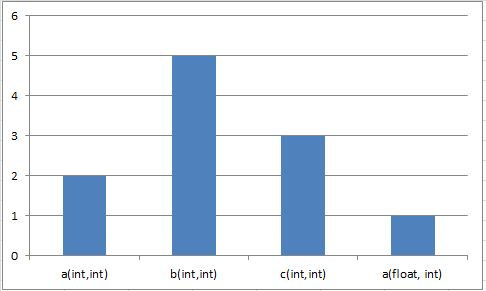
\includegraphics[width=8cm]{jit-1}
\end{figure}


\begin{figure}[h!]
  \caption{JIT compiler marking one of methods as hot and recompiling}
  \label{img:jit-2}
  \centering
	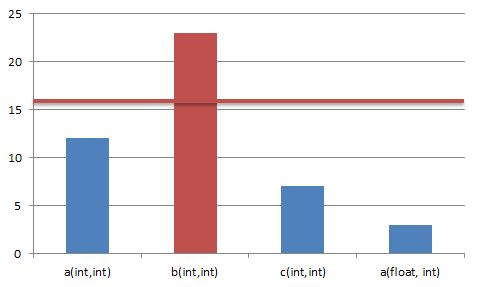
\includegraphics[width=8cm]{jit-2}
\end{figure}

This proved to be more effective and a simpler approach, which is now used in all JavaScript engines. In V8 Crankshaft, a step forward was taken, and simple methods are compiled even before any statistics on data types are collected. For compiled methods the source code is not stored. Instead, a procedure called deoptimisation is implemented. Whenever an engine detects that a compiled code does not match actual types of variables, the code is deoptimised and either optimised again to match the new, better set of variables, or kept in interpreter-friendly form.

To track these changes two debug options for V8 are available: --trace-opt and --trace-deopt.

\lstinputlisting[caption=Output from V8 debug run showing optimisation and deoptimisation,label=listing:optdeopt]{optdeopt.txt}


\section{Type inference}
\label{sec:typeference}

V8's method of optimising code before it is run relies on type inference. Based on the context of the variable its type is guessed. The generated assembler has to support cache miss -- whenever inferred type turns out to be incorrect, a new type is assigned and another JIT compilation runs. Types of variables are organised in a tree, where the Number object may store both Float or Integer, Integer may store SMI (small int), etc.

\lstinputlisting[caption=Tree of types in JavaScript,label=listing:typestree]{types.txt}

In V8 type inference is tightly connected with JIT compilation and may be tracked with the same flags: --trace-opt and --trace-deopt. 

\section{Hidden classes}
\label{sec:hiddenclasses}

JavaScript is a classless language. Object may have defined a prototype which behaves similar to base class in other langauges. However, a property may be added to an Object or its prototype at any point in runtime. To optimise such a dynamic representation, engines use the concept of hidden class. Whenever an Object is created, its hidden class is pointed to the base, empty Object representation. Then each definition of new property makes a transition on the hidden class graph, introducing hidden classes that are not yet defined, as in the following example:

\begin{figure}[h!]
  \caption{Initial shape of hidden class for Point}
  \label{img:point0}
  \centering
	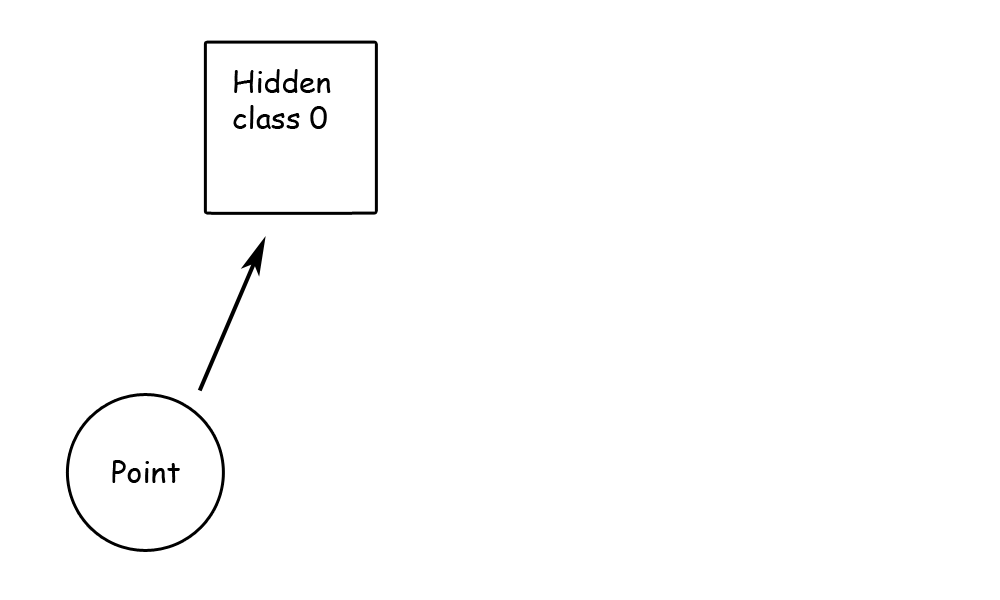
\includegraphics[width=8cm]{point0}
\end{figure}
\begin{figure}[h!]
  \caption{Shape of hidden class for Point after x property added}
  \label{img:point1}
  \centering
	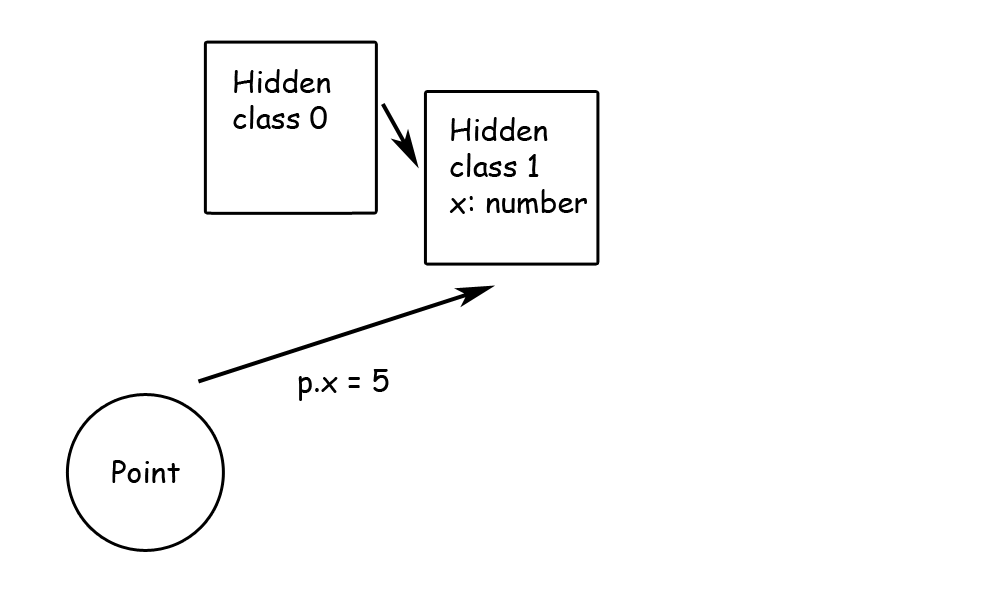
\includegraphics[width=8cm]{point1}
\end{figure}
\begin{figure}[h!]
  \caption{Shape of hidden class for Point after y property added}
  \label{img:point2}
  \centering
	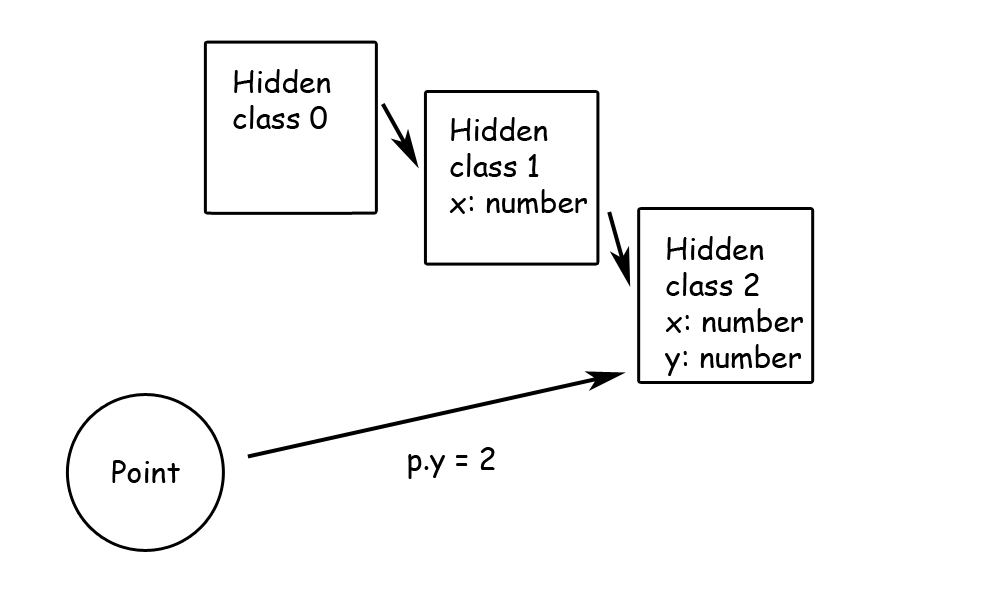
\includegraphics[width=8cm]{point2}
\end{figure}

Based on hidden class the JIT compiler optimises methods to generate an even simpler assembly code similar to the one compiled from C++. Class shape defines address offsets of Object properties. Thus, the hidden class graph is actually a tree, where one class cannot be reached in more than one way.

\begin{figure}[h!]
  \caption{Two point representations based on order of declared properties}
  \label{img:point_tree2}
  \centering
	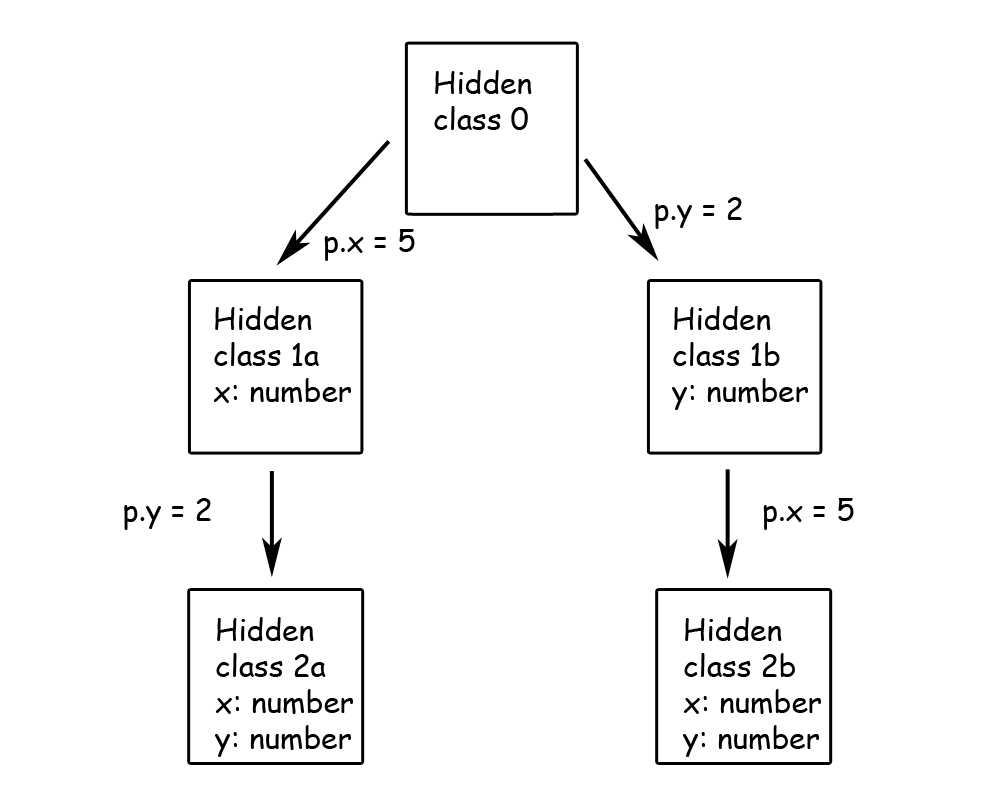
\includegraphics[width=8cm]{point_tree2}
\end{figure} 

At the moment of writing, the type of property is not tracked in hidden classes. The only exception are primitive values (see Listing \ref{listing:typestree}). In other words, storing an object in property results in the same hidden class, regardless of the hidden class of this object.

Transitions between hidden classes can be tracked in V8 using flags --trace-generalization tracking when variables are cast to a more generic type (e.g. SMI to Integer, or Integer to Number) and --trace-migration (tracking when hidden classes are migrated).

\lstinputlisting[caption=Log of migration trace in V8,label=listing:migration]{migration.txt}

\section{Garbage collection}
\label{sec:garbagecollection}

Memory in JavaScript is managed automatically. Each allocation places an object on a memory heap. The first generation of garbage collection traversed the whole tree and freed memory for all inaccessible objects. This type of deallocation is called mark-sweep and takes a long time. Since JavaScript is single-threaded, this operation blocks all other operations. To improve performance, especially in games, the incremental scavange method of garbage collection was introduced. The engine tracks the age of objects, allowing to quickly detect objects allocated temporarily (e.g. for a single frame rendered in a game). When the object is inaccessible, it is queued for deallocation, in chunks that do not cause long UI freezes.\footnote{http://en.wikipedia.org/wiki/Cheney's\_algorithm} \footnote{http://en.wikipedia.org/wiki/Garbage\_collection\_(computer\_science)}

\lstinputlisting[caption=Log of garbage collection in V8,label=listing:gc]{gc.txt}

\chapter{Particle system}
\label{cha:particlesystem}

Particle system is one of most commonly used techniques to simulate smoke, fire, rain and other groups of discrete objects, usually independent from each other. System consist of defined number of emitters, producing lightweight particle objects with certain parameters. Each emitter has defined production ratio and each particle a certain lifespan, resulting in upper limit of total particles on screen. Some systems use also attraction points which enable better control over particles, using equations often similar to those of electrostatic forces.
Such simulation is independent from rendering. The same particle system may be used for different effects with proper configuration.

\begin{figure}[h!]
  \caption{Example rendering of tested particle system}
  \label{img:particles}
  \centering
	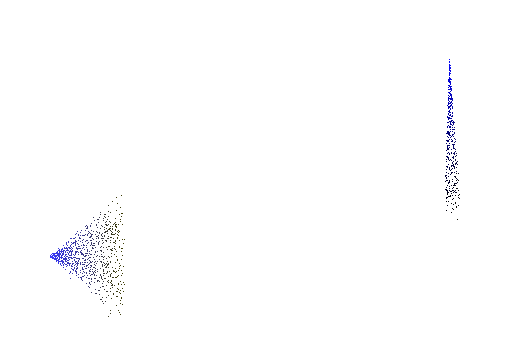
\includegraphics[width=16cm]{particles}
\end{figure}

\section{System parameters}
\label{sec:emittersparameters}

Tested system works on two-dimensional Cartesian plane. For purpose of  performance analysis movements are calculated based only on frames rather than actual flow of time. This means that systems with different framerate will result in different visualisations, but requesting given amount of frames rendered will result in the same lifespan and total number of particles in both systems.

Emitter supports following parameters:

\begin{itemize}
	\item position -- initial position of created particles
	\item angle -- angle counting clockwise from vector [0, 1]
	\item spread -- parameter controlling random differences in initial angle of particles
	\item velocity -- initial velocity of particles, in pixels per frame
	\item velocity spread -- parameter controlling random differences in initial velocity of particles
	\item lifespan -- initial lifespan of particles
	\item productionRate -- amount of particles initialized in each frame
\end{itemize}

A Particle has similar properties:
\begin{itemize}
	\item position
	\item velocity
	\item lifespan
	\item age -- counted in frames, when higher then lifespan particle is removed from system
\end{itemize}

Source code of both implementations is attached in Appendix \ref{cha:sourcecode}.

\section{Implementation with high memory allocation}
\label{sec:particlesinitial}

Initial tested implementation has one very important property of particle emitter. Whenever new particles are created, new array of pointers is allocated and returned from emitter. System appends new particles to existing array. In each frame particle system creates new, empty array of particles and adds there only particles that are still alive. Array from previous frame and all dead particles are removed from system and deallocated. This is clearly suboptimal solution that allocates and deallocates plenty of memory in each frame. Purpose of this exercise is to show how both languages handle bad code and how big impact it has comparing to the optimal solution.

TODO: this part may need to be updated before publication.
TODO: Is this accounting properly for v8 startup time? Maybe profiling ticks would be better.

\lstinputlisting[caption=Time measurement of unoptimized particle system in JavaScript,label=listing:timejs1]{particles/timejs1.txt}
\lstinputlisting[caption=Time measurement of unoptimized particle system in C++,label=listing:timecpp1]{particles/timecpp1.txt}

Time measurement shows that JavaScript version is almost 8 times slower than native one. To analyse situation --prof and --log-timer-events flags may be used. Output file v8.log is parsed using available online tool.\footnote{http://v8.googlecode.com/svn/branches/bleeding\_edge/tools/profviz/profviz.html}

\lstinputlisting[caption=Profiler output for unoptimized particles,label=listing:particles1profile]{particles/particles1-profile.txt}

Methods prefixed with ~ are unoptimized, the ones prefixed with * are JIT compiled. As seen in profiler log, most of the time is spent in unoptimised versions of verifyIfAlive and stepParticle methods of particle system step.

\lstinputlisting[caption=Annotated part of source,label=listing:particles1stepannotated,language=JavaScript]{particles/particleSystemstep.js}

The same methods are also used in optimised versions, where they take significantly less ticks to run. It's clear that presented code not only allocates and deallocates too much memory, but also fails to run in optimised mode. It's visible on chart obtained from the same tool -- stripe labelled "code kind in execution" shows multiple kinds of code running and is interrupted often with garbage collection cycles.

\begin{figure}[h!]
  \caption{Chart of time used in unoptimised verion of JavaScript}
  \label{img:particles1profile}
  \centering
	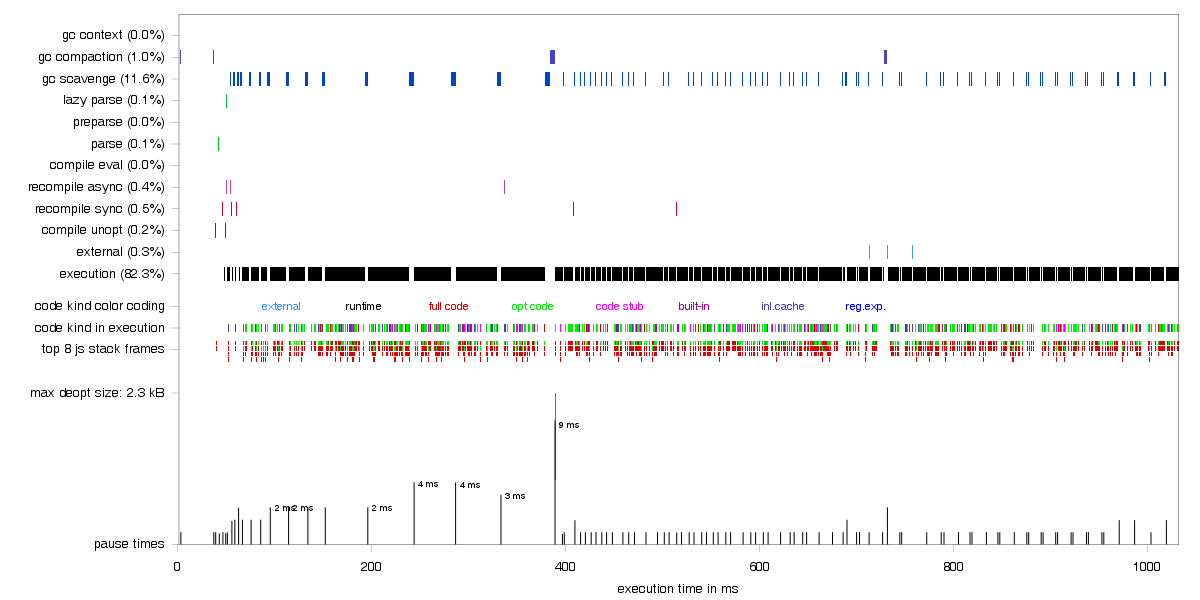
\includegraphics[width=16cm]{particles/particles1-profile.png}
\end{figure}

Garbage collection cycles blocking execution are also visible with --trace-gc flag.

\lstinputlisting[caption=Garbage collection in unoptimised particle system,label=listing:particles1gc]{particles/particles1gc.txt}

\section{Implementation with object pool}
\label{sec:particlesobjectpool}

To improve performance different approach to particles allocation is used. Each particle has a flag "isDead" telling if it may be safely reused for new particle. Particle pool is kept along with a list of pointers to dead particles. This way when system reaches it's maximum congestion (around 15000 particles in given example) no new allocations occur.
Creation of new particles is moved from particle emitter to particle system, to avoid allocation of new array. Emitter works now as a structure describing behaviour but not implementing one.

\lstinputlisting[caption=Time measurement of optimized particle system in JavaScript,label=listing:timejs2]{particles/timejs2.txt}
\lstinputlisting[caption=Time measurement of optimized particle system in C++,label=listing:timecpp2]{particles/timecpp2.txt}

Optimised version shows overall improvement of 85\% for JavaScript and 45\% for C++ making JavaScript version only 2.2 times slower than native one. It's clearly visible that JavaScript is more sensitive to unwise memory management.

\lstinputlisting[caption=Profiler output for optimized particles,label=listing:particles1profile]{particles/particles2-profile.txt}

Profiling shows that step method of particle system now runs always in optimised mode and almost no time is spent on other methods. The same is visible on profiling chart, where "code kind in execution" stripe shows only optimised code.

\begin{figure}[h!]
  \caption{Chart of time used in optimised verion of JavaScript}
  \label{img:particles2profile}
  \centering
	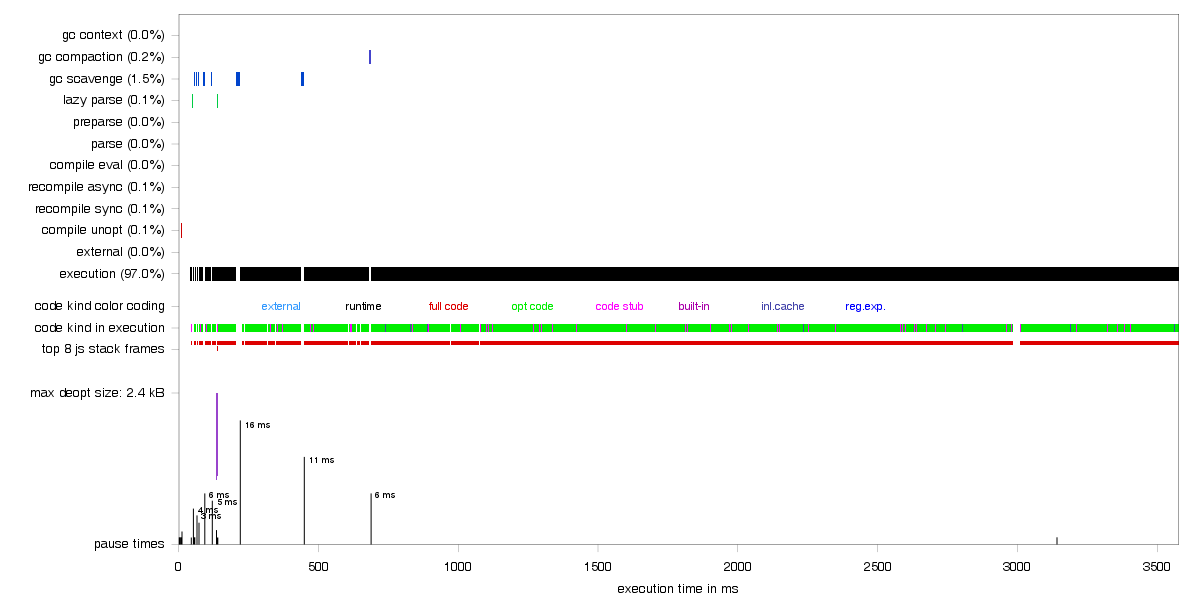
\includegraphics[width=16cm]{particles/particles2-profile.png}
\end{figure} 

Situation is also improved in garbage collection log.

\lstinputlisting[caption=Garbage collection in optimised particle system,label=listing:particles2gc]{particles/particles2gc.txt}

\chapter{Sphere collision}
\label{cha:spherecollision}

\section{Algorithm description}
\label{sec:spherealgorithmdescription}

\section{Three-dimensional SAT}

\section{{$O(N^2)$} approach}
\label{sec:sphereinitial}

\section{Octree-partitioned space}
\label{sec:sphereoctree}

\chapter{Emscripten}
\label{cha:emscripten}

JavaScript is often called an assembly language of the Web.\footnote{http://www.hanselman.com/blog/JavaScriptIsWebAssemblyLanguageAndThatsOK.aspx} One could argue that since only one language is supported by browsers it could be made a compilation target similar to assembler for CPU. This statement is flawed since eventually JavaScript is translated to assembly making it only an intermediate step. Probably resemblance to ByteCode in JVM, which is compilation target of multiple languages like Java, Scala and Clojure is more in place.
Nevertheless, last years showed multiple projects aimed at converting code to JavaScript. Some introduce new syntax like CoffeeScript, Dart or TypeScript while still serving the same purpose -- providing human readable code that is interpreted in browser on fly. Others, that are focus of this chapter, aim to convert existing projects to run in browser.

Several new projects are connected to make this happen. First steps in conversion between languages were made with LLVM project\footnote{http://llvm.org/} which currently is a collection of tools and compilers converting code to and from intermediate representation (LLVM IR). For C++ Clang\footnote{http://clang.llvm.org/} is a conversion tool.

\begin{figure}[h!]
  \caption{Pipeline of Emscripten conversion. Source: http://www.hanselman.com/blog/JavaScriptIsWebAssemblyLanguageAndThatsOK.aspx}
  \label{img:emscriptenpipeline}
  \centering
	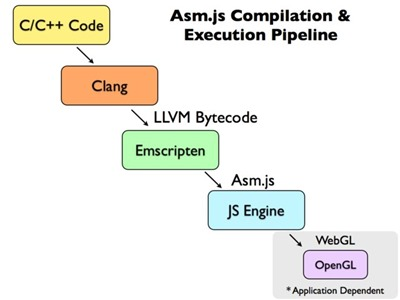
\includegraphics[width=8cm]{emscripten/pipeline.jpg}
\end{figure}

Code in LLVM is suitable for further conversion to language like JavaScript. This part is handled by Emscripten\footnote{https://github.com/kripken/emscripten/wiki} project. Initially compilation target for Emscripten was plain JavaScript. With recent developments asm.js\footnote{http://asmjs.org/spec/latest/} library was created. It provides syntax built on top of JavaScript, that is strongly typed and easily translatable to assembly language. Asm.js details are explained in section \ref{sec:asmjsoverview}.

\lstinputlisting[caption=Example of code using asm.js,label=listing:asmjs]{emscripten/asm.js}

Project, built in cooperation with Mozilla Foundation, has its own engine for Firefox -- OdinMonkey, designed to run faster for this limited and well-defined syntax.

Altogether these projects resulted in multiple libraries and games converted from native version to JavaScript.

Proof-of-concept demo made in cooperation between Mozilla and Unreal is Epic Citadel HTML5 -- Unreal Engine 3 technology demo\footnote{http://www.unrealengine.com/en/showcase/udk/epic\_citadel/}  instance running in browser.\footnote{http://www.unrealengine.com/html5/} Companies claim it took only four days to complete the conversion.

\begin{figure}[h!]
  \caption{Epic Citadel screenshot}
  \label{img:epicitadel}
  \centering
	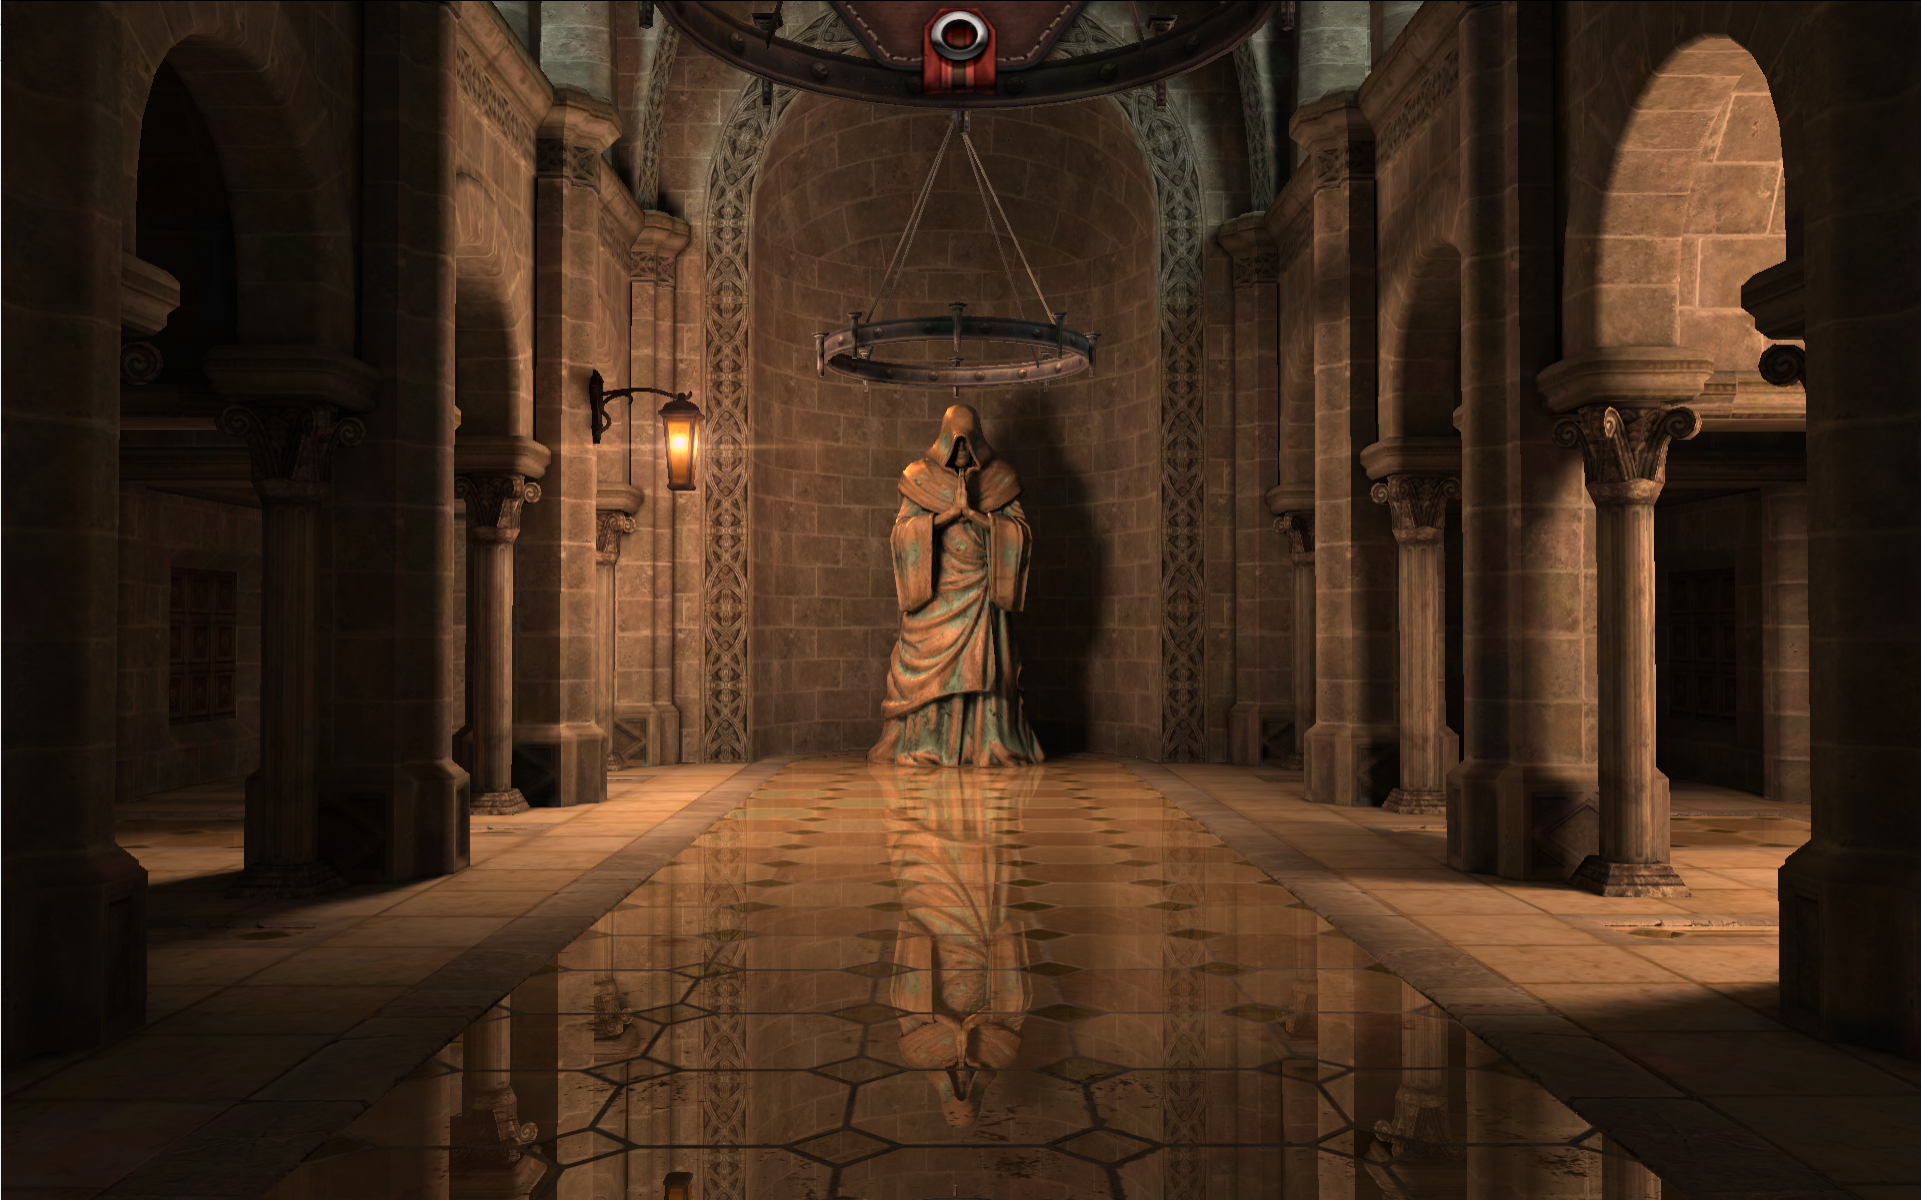
\includegraphics[width=16cm]{emscripten/epic-citadel.jpg}
\end{figure}

Another example of successful converted project is ammo.js\footnote{https://github.com/kripken/ammo.js/} -- originating from Bullet physics engine.
TODO: Maybe extend this part a bit, cover more on how conversion was going and what were the issues.

\begin{figure}[h!]
  \caption{Ammo.js demo colliding 500 boxes at 30fps, available at http://kripken.github.io/ammo.js/examples/new/ammo.html}
  \label{img:epicitadel}
  \centering
	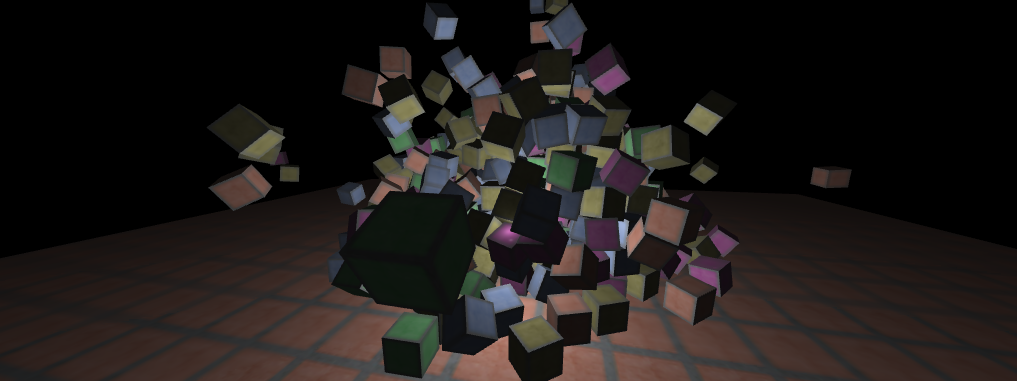
\includegraphics[width=16cm]{emscripten/ammojs.png}
\end{figure}

\section{Asm.js overview}
\label{sec:asmjsoverview}

Asm.js introduces some improvements targeted to fix performance problems of JavaScript. Ahead of time compilation enforces very specific rules on coding style. Documentation\footnote{http://asmjs.org/spec/latest/} lists:

\subsection{Unboxed representations of integers and floating-point numbers}
\label{sec:asmjsunboxed}
In asm.js only types allowed are integers and doubles. All numbers have annotations indicating static type (see: \ref{listing:typestree}). This way compiler doesn't have to detect possible transitions between variable types and code overall runs faster.

\subsection{Absence of runtime type checks}
\label{sec:asmjstypechecks}
Since asm.js works only on well-defined numbers, all function calls are monomorphic and stable. In OdinMonkey ahead-of-time compilation is able to compile them to the most optimised version without tracking method calls. In engines using JIT methods are compiled early and newer deoptimised.

\subsection{Absence of garbage collection}
\label{sec:asmjsgc}
As shown in previous chapters, garbage collection calls are often a performance bottleneck. Asm.js solves this problem by eliminating garbage collection completely. Memory is stored in short-life variables, deallocated after method exits and in global heaps, which are never resized or deallocated.

\subsection{Efficient heap loads and stores}
\label{sec:asmjsheap}

Heaps are global arrays of statically typed arrays, in JavaScript implemented as objects listed in \ref{table:jsarrays}. Size of heap doesn't change during runtime -- it has to be calculated during compilation and incorrect prediction or memory leaks may result in buffer overflow. Heaps are always passed as an argument to asm.js modules. Each module may reference part of the heap and use it as long as necessary.

\begin{table}[h!]
\caption{Statically typed arrays in JavaScript}
\centering
\label{table:jsarrays}
\begin{tabular}{|l|l|l|}
  	\hline
View Type & Element Size (Bytes) & Element Type \\ \hline
Uint8Array & 1 & intish \\ \hline
Int8Array & 1 & intish \\ \hline
Uint16Array & 2 & intish \\ \hline
Int16Array & 2 & intish \\ \hline
Uint32Array & 4 & intish \\ \hline
Int32Array & 4 & intish \\ \hline
Float32Array & 4 & doublish \\ \hline
Float64Array & 8 & doublish \\ \hline
\end{tabular}
\end{table}

\subsection{Summary}
\label{sec:asmjssummary}

These solutions remove some of performance bottlenecks described in previous chapters. Code suitable to run with asm.js is almost unreadable by programmer and resembles assembly code. Asm.js is not designed to be a language used by a programmer, it is mainly a target for compilation using converters like Emscripten. 

Most of optimisation used by asm.js are consistent with code that is expected by V8 engine -- variables and methods are monomorphic, garbage collection is close to zero. It's worth noting that code written by hand is almost always shorter that one generated by Emscripten. Partial solution for this is built-in Google Closure Compiler used on output of Emscripten and different levels of optimisation.
In tests mentioned in this work all solutions take 2 to 4kB compiled, while Emscripten produces over 450kB of code for each. This affects real life performance by lengthening at least transfer and parse time for code. Average parse time of 1kB of JS is believed to be up to 1ms\footnote{https://developers.google.com/speed/docs/best-practices/mobile}. Global average bandwidth was 3.1 Mbps in Q1 2013\footnote{http://www.akamai.com/dl/akamai/akamai\_soti\_q113.pdf} thus transfer of each kilobyte is around 2.5ms. In total, load time of tested code is approximately 1.5 second on average bandwidth and platform. In case of larger applications and games waiting time for load may be significantly larger and should be taken under consideration.

\chapter{Summary}
\label{cha:summary}

Conducted experiments show a gap between JavaScript and C++ performance. Significant language design differences result in code that is often easier to write but also easier to abuse. Benchmarks show differences between 15\% and 100\% overhead for correctly designed JavaScript code and over 500\% for incorrect patterns.  Considering Moore's law stating that computers double speed every 18 months it safe to say that JavaScript is very close to being suitable for any type of development. 

Conducted experiments show clear pattern regarding dynamic variable types in JavaScript. Whenever boxing and unboxing happens, JIT compilation is not able to properly optimise code and bring it up to performance of C++. This affects both simple variables and properties end is especially visible for numbers. Transitions between integer and floats are expensive while easy to overlook.

Types affect significantly also method calls cost. Keeping methods monomorphic in core parts of physics engine is very important. Additional cost of polymorphism of parameters is not only boxing and unboxing of parameters but also time spent of optimising and deoptimising compiled method which makes initial warmup of engine longer. Exporting well defined methods to be called from polymorphic ones is an easy workaround for this performance bottleneck.

Lastly, memory management proven to be one of the most important problems in JavaScript. Automated garbage collection connected with popular pattern of creating and returning of arrays is an important problem. Memory allocation of objects is also a bottleneck, but not very dissimilar to one in C++. As shown in second version of particle system, usage of object pools and changing architecture to avoid array creation are techniques that can be employed to fight with it. It is worth mentioning that while garbage collection always introduces some overhead it is reasonable to avoid it at all costs. Sphere collision system with octree partitioning is also introducing and destroying objects, but overhead is significantly smaller than gained speedup. Advice for memory operations is to avoid objects living only for a single frame i.e. temporary variables and helpers. Long living objects are in general unavoidable and should be used whenever suitable.

General advice for programming in JavaScript is to use techniques similar to those found in asm.js - keep types static, method calls monomorphic and work carefully with memory.

Conducted tests show that while gap between JavaScript and native application exists and is not insignificant, there is a lot of potential in such approach. It is expected, that with growing community and interest from game industry new games will be released on browser within few years. Performance issues may prevent works on AAA titles, but companies focused more on social aspect of games and new trends in monetisation may create games targeted for different users. With capabilities of browsers equal to having 18 months older machine, less graphically demanding titles like The Sims or World or Warcraft may certainly be ported to run in JavaScript.


\appendix
\chapter{Acknowledgements}
\label{cha:acknowledgements}



\chapter{Source code}
\label{cha:sourcecode}


\section{Math utilities}
\label{sec:mathsource}

\lstinputlisting[caption=Math utilities in JavaScript,label=listing:mathjs,language=JavaScript]{math.js}
\lstinputlisting[caption=Math utilities in C++,label=listing:mathjs,language=C++]{math.cpp}

\section{Particle system}
\label{sec:particlesource}

\lstinputlisting[caption=Particle object in JavaScript,label=listing:particlejs,language=JavaScript]{particles/particle.js}
\lstinputlisting[caption=Particle object in C++,label=listing:particlejs,language=C++]{particles/particle.cpp}
\lstinputlisting[caption=Particle emitter object in JavaScript,label=listing:particleemitterjs,language=JavaScript]{particles/particleEmitter.js}
\lstinputlisting[caption=Particle emitter object in C++,label=listing:particleemittercpp,language=C++]{particles/particleEmitter.cpp}
\lstinputlisting[caption=Initial particle system object in JavaScript,label=listing:particlesystem1js,language=JavaScript]{particles/particleSystem.js}
\lstinputlisting[caption=Initial particle system in C++,label=listing:particlesystem1cpp,language=C++]{particles/particleSystem.cpp}
\lstinputlisting[caption=Optimised particle system object in JavaScript,label=listing:particlesystem2js,language=JavaScript]{particles/particleSystem2.js}
\lstinputlisting[caption=Optimised particle system in C++,label=listing:particlesystem2cpp,language=C++]{particles/particleSystem2.cpp}


\section{Spheres collision detection}
\label{sec:spheressource}

\lstinputlisting[caption=Sphere object in JavaScript,label=listing:spherejs,language=JavaScript]{spheres/sphere.js}
\lstinputlisting[caption=Sphere object in C++,label=listing:spherejs,language=C++]{spheres/sphere.cpp}

\lstinputlisting[caption=Sphere system object in JavaScript,label=listing:spheresystemjs,language=JavaScript]{spheres/sphereSystem.js}
\lstinputlisting[caption=Sphere system in C++,label=listing:spheresystemcpp,language=C++]{spheres/sphereSystem.cpp}


\lstinputlisting[caption=Octree in JavaScript,label=listing:octreejs,language=JavaScript]{spheres/octree.js}
\lstinputlisting[caption=Octree in C++,label=listing:octreecpp,language=C++]{spheres/octree.cpp}


\lstinputlisting[caption=Octree-based sphere system object in JavaScript,label=listing:spheresystem2js,language=JavaScript]{spheres/sphereSystem2.js}
\lstinputlisting[caption=Octree-based sphere system in C++,label=listing:spheresystem2cpp,language=C++]{spheres/sphereSystem2.cpp}


\clearpage
\phantomsection
\addcontentsline{toc}{chapter}{References}
\nocite{*}
\bibliographystyle{ieeetr}
\bibliography{bibliografia}

\end{document}
 
